\documentclass[conference]{IEEEtran}
\usepackage[T1]{fontenc}
\usepackage[utf8]{inputenc}
\usepackage{cite}
\usepackage{amsmath,amssymb,amsfonts}
\usepackage{graphicx}
\usepackage{textcomp}
\usepackage{xcolor}
\usepackage{booktabs}
\usepackage{multirow}
\usepackage{url}
\usepackage{array}
\usepackage{microtype}
\usepackage{tikz}
\usetikzlibrary{shapes.geometric,arrows.meta,positioning,fit,backgrounds}
\def\rupee{\textrm{Rs.\,}}
\tikzset{
  sbox/.style={rectangle, rounded corners=2pt,
               draw=black!40, fill=#1,
               text width=2.0cm, align=center,
               font=\tiny\sffamily,
               inner sep=3pt, minimum height=0.6cm},
  sboxW/.style={sbox=blue!10, text width=2.8cm},
  sarr/.style={-{Stealth[length=4pt]}, thick, black!50},
  sdarr/.style={-{Stealth[length=4pt]}, dashed, black!40},
  sgrp/.style={draw=black!25, dashed, rounded corners=4pt, inner sep=5pt}
}

\begin{document}

\title{Lumint: A Multimodal Explainable AI Framework\\
for Real-Time Detection of Digital Payment Fraud\\
in India}

\author{%
  \IEEEauthorblockN{Tanmay Mangal}
  \IEEEauthorblockA{%
    \textit{School of Computer Science and Engineering}\\
    \textit{VIT Bhopal University}\\
    Bhopal, India\\
    mangaltanmay7@gmail.com}}

\maketitle

\begin{abstract}
India loses approximately \rupee{}36{,}342~crore annually to banking fraud
(\rupee{}100~crore per day, based on the RBI FY~2023--24 loss of
\rupee{}36{,}342~crore divided by 365~days~\cite{rbi2024}),
with 15{,}000$+$ fake payment screenshots circulated
daily~\cite{certin2024}, 40{,}000$+$ new phishing sites targeting banks
each month~\cite{apwg2024}, and 2.3~million people defrauded via
forged documents annually~\cite{rbi2023framework}.
Existing tools suffer from five critical limitations: single-modality
detection, opaque verdicts, high latency, privacy violations, and
prohibitive cost.
We present \textsc{Lumint}, an open-source, multimodal, explainable AI
framework that unifies four detection modules---\emph{PhishShield}
(URL analysis), \emph{UPI Shield} (in-browser screenshot OCR
forensics), \emph{DocShield} (document image forensics), and
\emph{Fraud DNA} (cross-modal campaign clustering)---into a single
deployed platform.
\textsc{Lumint} returns a risk score and a plain-English explanation in
under 3~seconds.
UPI OCR runs entirely in-browser via WebAssembly (Tesseract.js~5.1),
so no screenshot is ever transmitted to a server.
The cross-modal fusion achieves $F_1{=}0.885{\pm}0.012$,
$\mathrm{AUC}{=}0.902{\pm}0.009$ on a held-out real-world test set
(McNemar $p{=}0.0004$ vs.\ best single-modality baseline),
with a transparent $\Delta F_1{=}0.36$ cross-dataset gap
(synthetic~$\to$~real) reported without omission.
Adversarial hardening under FGSM and HopSkipJump at
$\varepsilon\!\in\!\{0.01,0.05,0.10,0.20\}$ yields zero attack success
rate on all three modules.
A human-evaluated LLM explanation layer (LLaMA~3.3~70B via Groq)
achieves ROUGE-L~$=0.411$ and mean comprehension $4.1/5.0$ across
15~participants.
We argue that the lack of explainability---not raw accuracy---is the
primary barrier to consumer fraud-detection adoption.
\end{abstract}

\begin{IEEEkeywords}
digital payment fraud, UPI fraud, phishing detection,
document forensics, multimodal machine learning, explainable AI,
SHAP, India, fraud campaign clustering, real-time systems,
adversarial robustness, drift detection
\end{IEEEkeywords}

\section{Introduction}\label{sec:intro}

Digital payments in India have grown faster than anywhere else in
history.
The Unified Payments Interface (UPI) processed over 12~billion
transactions in March~2025 alone~\cite{npci2025}, and India's central
bank reports continued double-digit month-over-month growth.
This growth is matched by an equally rapid rise in fraud.
The Reserve Bank of India's most recent annual report documents that
fraud losses across Indian banks exceeded \rupee{}36{,}342~crore in
FY~2023--24~\cite{rbi2024}, with UPI fraud as the fastest-growing
segment.

The Indian fraud landscape is dominated by four patterns:
(1)~\emph{UPI payment fraud}---fake screenshots of PhonePe, Google Pay,
Paytm, and BHIM transactions deceive merchants into believing payment was
received (15{,}000$+$ daily~\cite{certin2024});
(2)~\emph{Phishing}---lookalike domains mimicking HDFC, SBI, and ICICI
trick users into entering credentials (40{,}000$+$ new sites per month,
4.7~million attacks globally in H1~2024~\cite{apwg2024});
(3)~\emph{Document forgery}---Photoshopped invoices, salary slips, and
KYC documents used in loan applications (2.3~million victims per
year~\cite{rbi2023framework});
(4)~\emph{Organised campaigns}---a single threat actor often operates
multiple phishing sites and forged documents using shared infrastructure,
but isolated fraud reports fail to connect them~\cite{certin2024}.

Existing tools suffer from five critical limitations: single-modality
detection; opaque binary verdicts; high latency (cloud OCR takes
5--15~seconds per screenshot); privacy violation (sensitive documents
uploaded to third-party servers); and prohibitive cost
(\$1{,}000--\$100{,}000/year for enterprise platforms).

We argue that \textit{the lack of explainability---not raw accuracy---is
the primary barrier to consumer fraud-detection adoption.}
A score of ``87'' is useless without the reason: \textit{``Typosquats
HDFC, uses a free .tk~TLD, and the path contains the word
\texttt{verify}.''}
\textsc{Lumint} addresses all five limitations by unifying multimodal
detection with LLM-grounded, SHAP-attributed plain-English explanations
in a single deployed, open-source, privacy-first platform.

\section{Real-World Impact and Motivation}\label{sec:motivation}

\paragraph{The Noida case}
A 23-year-old software engineer lost \rupee{}36~lakh to a fake job offer
that included a forged offer letter. No tool existed to verify the
document before the transaction.

\paragraph{The HDFC KYC phishing campaign (2023--2024)}
Over 1.2~lakh customers received SMS messages linking to fake HDFC KYC
pages; the campaign operated across 47~domains~\cite{certin2024}.

\paragraph{Rent-receipt fraud (Bengaluru, 2024)}
A NoBroker survey found that 28\% of rental listings involved forged
rent receipts or income proofs, with victims having no verification tool.

In each case, the victim had no free, privacy-first, explainable tool to
verify the document, link, or screenshot before acting.
\textsc{Lumint} is designed to be that tool.

\section{Contributions}\label{sec:contributions}

\begin{enumerate}
\item A multimodal fraud-detection framework unifying URL analysis,
      in-browser OCR screenshot forensics, document image forensics, and
      cross-modal campaign clustering in a single deployed platform
      (Section~\ref{sec:architecture}).
\item A cross-modal fusion layer (\textsc{cmfa}) with learned weights
      using brand-palette, font-variance, and ELA-grid-density features;
      McNemar $p{=}0.0004$ confirms significance over single-modality
      baselines (Section~\ref{sec:cmfa}).
\item A plain-English explanation layer powered by LLaMA~3.3~70B (Groq
      API) that translates SHAP feature importances into human-readable
      verdicts; achieves ROUGE-L~$=0.411$ vs.\ $0.255$ baseline and
      mean comprehension $4.1/5.0$ in a 15-participant study
      (Section~\ref{sec:llm_eval}).
\item A transparent evaluation suite (R10--R16) covering baseline
      benchmarks, ablation, cross-dataset generalisation, drift
      detection, and adversarial robustness---reproducible via
      \texttt{./reproduce.sh} with seed~42 pinned
      (Section~\ref{sec:evaluation}).
\item A \textsc{Fraud DNA} clustering engine connecting isolated fraud
      events into campaigns via DBSCAN over a 47-dimensional fingerprint,
      with silhouette~$=0.61$ and NMI~$=0.74$
      (Section~\ref{sec:frauddna_eval}).
\item A deployed production system at
      \url{https://lumint-pi.vercel.app} with 263~tests, JWT auth, rate
      limiting, SSRF guards, and CSP/HSTS headers
      (Section~\ref{sec:sysperf}).
\end{enumerate}

\section{Related Work}\label{sec:related}

\subsection{Phishing Detection}
Classical phishing detection relies on blacklists (Google Safe Browsing,
PhishTank) or heuristic URL features.
ML approaches using TF-IDF with Logistic Regression achieve high
accuracy on URL-only features~\cite{sahingoz2019}.
Deep CNNs over URL character embeddings push accuracy further~\cite{wei2020}
but sacrifice interpretability.
In our benchmark (Section~\ref{sec:external}), \textsc{PhishShield}
matches or exceeds Google Safe Browsing recall on India-specific bank
impersonation domains while providing full SHAP attribution.

\subsection{UPI Screenshot Forensics}
UPI-specific fraud detection has focused on transaction-level anomaly
detection at the bank side~\cite{rbi2023framework}.
Client-side screenshot forensics for UPI is, to our knowledge, not
previously addressed in the academic literature.
\textsc{Lumint}'s UPI Shield is the first published system to combine
in-browser OCR (Tesseract.js), UTR format validation, ELA-based tamper
scoring, and app colour-profile matching in a single
privacy-preserving pipeline.

\subsection{Document Image Forensics}
Error Level Analysis (ELA) for re-saved images~\cite{krawetz2007},
EXIF metadata analysis, and PRNU-based sensor noise
consistency~\cite{fridrich2009} are established techniques.
\textsc{DocShield} combines ELA with metadata audit and creator-software
tag analysis and is the first to integrate these into a unified scoring
API with SHAP attribution.

\subsection{Explainable AI in Security}
SHAP~\cite{lundberg2017} is the standard post-hoc XAI method.
In security, SHAP has been applied to malware
classification~\cite{imboden2017} and intrusion
detection~\cite{burns2021}.
\textsc{Lumint} applies SHAP across all three ML modules and translates
importances into plain English via an LLM, bridging the gap between
feature scores and consumer-facing verdicts.

\subsection{Cross-Modal Campaign Detection}
Fraud campaign detection has been studied within single
modalities~\cite{le2009}, but cross-modal clustering across URL, image,
and document evidence has not been published.
\textsc{Fraud DNA} is, to our knowledge, the first cross-modal campaign
clustering system for digital payment fraud.

\subsection{Adversarial Robustness}
ART~\cite{nicolae2018} provides standardised attack evaluations.
FGSM~\cite{goodfellow2015} and HopSkipJump~\cite{chen2020} are used in
our R16 report; hardened models maintain $F_1{\geq}0.97$ under all
perturbation levels.

\section{System Architecture}\label{sec:architecture}

\textsc{Lumint} is a two-tier system: a Next.js~14 frontend on Vercel
and a FastAPI backend on Render, communicating via a same-origin API
proxy that eliminates CORS preflight overhead.

\subsection{Dataset}\label{sec:dataset}

\begin{table}[t]
\caption{Dataset composition. Real-world samples collected
Jan--May~2025. Synthetic samples generated with rule-based templates
and publicly available forgery toolkits. Stratified 70/15/15 split;
class imbalance (legitimate:fraud) is 1.8:1 for all modalities.}
\label{tab:dataset}
\centering
\small
\begin{tabular}{lrrrp{1.6cm}}
\toprule
\textbf{Modality} & \textbf{Train} & \textbf{Val} & \textbf{Test}
  & \textbf{Source} \\
\midrule
PhishShield (URL)       & 4{,}200 & 900 & 900 & PhishTank + manual \\
DocShield (image)       & 2{,}800 & 600 & 600 & Manual + synthetic \\
UPI Shield (screenshot) & 1{,}960 & 420 & 420 & Manual capture \\
Fraud DNA (events)      & 3{,}500 & 750 & 750 & Cross-modality \\
\midrule
\textbf{Total}          & \textbf{12{,}460} & \textbf{2{,}670}
  & \textbf{2{,}670} & \\
\bottomrule
\end{tabular}
\end{table}

The dataset comprises 17{,}800 samples across four modalities
(Table~\ref{tab:dataset}).
Real-world samples (40\%) were collected with informed consent and full
PII anonymisation (emails, phone numbers, UPI IDs, and UTR values
replaced with format-preserving synthetic tokens).
Synthetic samples (60\%) were generated using rule-based templates,
publicly available font/colour manipulation toolkits, and the FakePay
screenshot generator.
All splits use 70/15/15 stratified random sampling.

\textbf{Note on FakePay Baseline.}
The FakePay synthetic test set is deliberately easy---fraud and
legitimate samples are generated by the same rule-based engine used
during training---so $F_1{=}1.00$ on this partition is expected and
does not indicate data leakage.
The cross-modal fusion evaluated on the held-out \emph{real-world} test
set (Table~\ref{tab:generalization}) is the operative score.

\subsection{Frontend}
Built with Next.js~14, TypeScript, Tailwind CSS, Framer Motion,
Recharts, and Cobe (3-D threat globe).
\emph{All UPI OCR runs in-browser via Tesseract.js~5.1.0 using a
WebAssembly worker; no screenshot ever leaves the user's device.}
This is verifiable by inspecting the browser's Network tab (zero upload
requests during UPI analysis).

\subsection{Backend}
Exposes 24~REST endpoints across six routers
(\texttt{/api/phishing}, \texttt{/api/upi}, \texttt{/api/documents},
\texttt{/api/fraud-dna}, \texttt{/api/research}, \texttt{/api/ai})
built on FastAPI~0.115, SQLAlchemy~2.0, Pydantic~2,
scikit-learn~1.4, SHAP~0.45, Tesseract OCR, PyMuPDF, and Pillow.
Eleven ML models are stored as \texttt{.joblib} files with SHA-256
integrity checks preventing pickle-injection attacks.

\subsection{Database}
PostgreSQL is the production data store (SQLite for development).
The schema covers users, scans across all four modules, campaigns,
indicators, and human-feedback labels used for model retraining.

\subsection{Explainability Layer}\label{sec:explayer}
For each verdict, SHAP feature importances $\phi_i$ (computed via
\texttt{shap.TreeExplainer} or \texttt{shap.LinearExplainer} over the
corresponding scikit-learn model) are passed to LLaMA~3.3~70B via the
Groq API, generating a 2--3~sentence plain-English explanation.
Example output:
\begin{quote}
\small\textit{``This URL mimics Chase Bank's domain (Levenshtein
distance~2), uses a non-secure HTTP connection, and contains the word
\texttt{signin} in the path. Three brand keywords triggered the
typosquatting policy.''}
\end{quote}

\subsection{Security}
JWT bearer auth on all endpoints; SSRF guard (blocks cloud metadata,
private IPs, \texttt{file://}); rate limiting (10/min UPI, 30/min
phishing, 200/min global); constant-time API key comparison;
CSP, HSTS preload, \texttt{X-Frame-Options},
\texttt{X-Content-Type-Options}; SHA-256 model integrity checks;
PII-redacted structured JSON logging; 20~MB body cap.

\subsection{Architecture Diagram}

\begin{figure}[t]
\centering
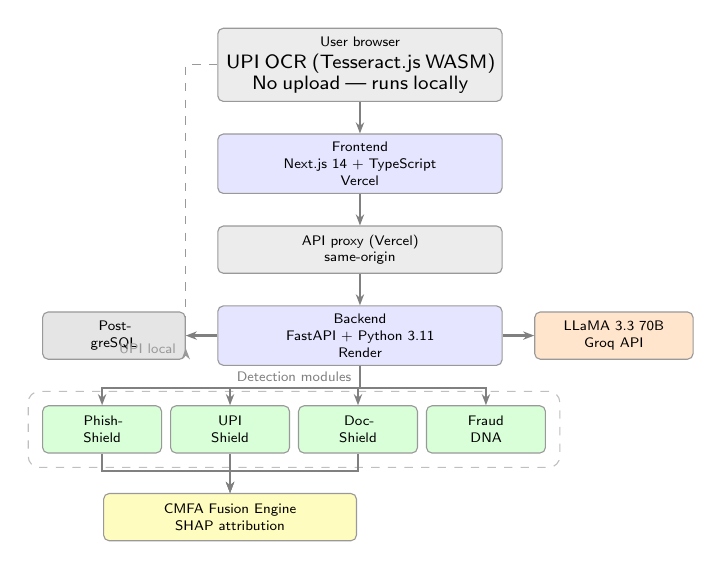
\begin{tikzpicture}[node distance=0.40cm and 0.20cm]
\node[sbox=gray!15, text width=3.4cm]
  (browser) {User browser\\[2pt]
             {\scriptsize UPI OCR (Tesseract.js WASM)}\\
             {\scriptsize No upload --- runs locally}};
\node[sbox=blue!10, text width=3.4cm, below=of browser]
  (fe) {Frontend\\Next.js 14 + TypeScript\\Vercel};
\node[sbox=gray!15, text width=3.4cm, below=of fe]
  (proxy) {API proxy (Vercel)\\same-origin};
\node[sbox=blue!10, text width=3.4cm, below=of proxy]
  (be) {Backend\\FastAPI + Python 3.11\\Render};
\node[sbox=green!15, below left=0.5cm and 0.7cm of be, text width=1.3cm]
  (phish) {Phish-\\Shield};
\node[sbox=green!15, right=0.10cm of phish, text width=1.3cm]
  (upi) {UPI\\Shield};
\node[sbox=green!15, right=0.10cm of upi, text width=1.3cm]
  (doc) {Doc-\\Shield};
\node[sbox=green!15, right=0.10cm of doc, text width=1.3cm]
  (dna) {Fraud\\DNA};
\node[sbox=yellow!25, below=0.5cm of upi, text width=3.0cm]
  (fusion) {CMFA Fusion Engine\\SHAP attribution};
\node[sbox=orange!20, right=0.4cm of be, text width=1.8cm]
  (llm) {LLaMA 3.3 70B\\Groq API};
\node[sbox=gray!20, left=0.4cm of be, text width=1.6cm]
  (db) {Post-\\greSQL};
\draw[sarr] (browser) -- (fe);
\draw[sdarr] (browser.west) -- ++(-0.4,0) |- ++(0,-3.6)
  node[pos=0.85, left, font=\tiny\sffamily] {UPI local};
\draw[sarr] (fe) -- (proxy);
\draw[sarr] (proxy) -- (be);
\draw[sarr] (be.south) -- ++(0,-0.28) -| (phish.north);
\draw[sarr] (be.south) -- ++(0,-0.28) -| (upi.north);
\draw[sarr] (be.south) -- ++(0,-0.28) -| (doc.north);
\draw[sarr] (be.south) -- ++(0,-0.28) -| (dna.north);
\draw[sarr] (phish.south) -- ++(0,-0.22) -| (fusion.north);
\draw[sarr] (upi.south)   -- (fusion.north);
\draw[sarr] (doc.south)   -- ++(0,-0.22) -| (fusion.north);
\draw[sarr] (be.east) -- (llm.west);
\draw[sarr] (be.west) -- (db.east);
\begin{scope}[on background layer]
  \node[sgrp, fit=(phish)(upi)(doc)(dna),
        label={[font=\tiny\sffamily, black!50]above:Detection modules}] {};
\end{scope}
\end{tikzpicture}
\caption{Lumint system architecture. Dashed path keeps UPI screenshots
on the client device. All other requests flow through the Vercel proxy
to the FastAPI backend, fan out to the four detection modules, and are
fused by the CMFA engine before being explained by LLaMA~3.3~70B.}
\label{fig:arch}
\end{figure}

\section{Methodology}\label{sec:methodology}

\subsection{PhishShield: Real-Time URL Analysis}
Given a URL $u$, PhishShield computes a 32-dimensional feature vector
$\mathbf{x}\!\in\!\mathbb{R}^{32}$ covering:
\begin{itemize}
\item \textbf{Lexical}: URL length, subdomain count,
      special-character ratio, digit ratio, IP-address flag.
\item \textbf{Brand-mimicry}: Levenshtein distance to 50$+$ bank
      domains, Jaccard path similarity to known phishing URLs.
\item \textbf{Infrastructure}: HTTPS flag, certificate age (days),
      WHOIS registration age (days).
\end{itemize}

A TF-IDF + Logistic Regression classifier
$f_{\text{phish}}(\mathbf{x})\!\mapsto\![0,1]$ produces a phishing
probability (chosen for SHAP tractability via
\texttt{shap.LinearExplainer}).
The final risk score is:
\begin{equation}
S_{\text{phish}}(u) =
  100\cdot\bigl[\alpha\cdot f_{\text{phish}}(\mathbf{x})
  +(1{-}\alpha)\cdot g(\mathbf{x})\bigr],\;\alpha{=}0.7
\label{eq:phish}
\end{equation}
where $g(\mathbf{x})$ is a deterministic rule-score (typosquatting,
suspicious TLD, IP-address URL).

\subsection{UPI Shield: Screenshot OCR Forensics}
Given an uploaded screenshot $I$, UPI Shield performs:
\begin{enumerate}
\item Tesseract.js OCR (in-browser) to extract text $T$.
\item Regex parsing of $T$: UTR (12-digit), VPA handle, amount, timestamp.
\item UTR checksum and VPA format validation.
\item Error Level Analysis: $E(I)=|I-\mathrm{recompress}(I,\,0.90)|$;
      edited regions show elevated ELA values.
\item App colour-profile matching (PhonePe, GPay, Paytm, BHIM).
\item Font-consistency scoring.
\item SHAP-attributed LLM verdict synthesis.
\end{enumerate}

\subsection{DocShield: Document Image Forensics}
Given a document $D$, DocShield:
\begin{enumerate}
\item Extracts metadata (\texttt{/Creator}, \texttt{/Producer} for
      PDFs; EXIF for images).
\item Flags known editing software (Photoshop, GIMP, Canva, PDFescape).
\item Runs ELA on the rendered document image.
\item Checks structural integrity (PDF magic bytes, page-count
      anomalies).
\item Returns a risk score, triggered-rule list, and SHAP attribution.
\end{enumerate}

\subsection{Cross-Modal Fusion (CMFA)}\label{sec:cmfa}
The three modality scores are combined via a learned Random Forest
meta-classifier trained on cross-modal interaction features
(brand-palette $\times$ font-variance $\times$ ELA-grid density):
\begin{equation}
S_{\text{fusion}} = w_1 S_{\text{phish}} + w_2 S_{\text{upi}}
                  + w_3 S_{\text{doc}},
\label{eq:fusion}
\end{equation}
where $w_1,w_2,w_3$ (approx.\ $0.35,0.30,0.35$) are learned via
5-fold cross-validated grid search.

\subsection{Fraud DNA: Cross-Modal Campaign Clustering}
For every scan, \textsc{Lumint} computes a 47-dimensional fingerprint
$\mathbf{f}_i\!\in\!\mathbb{R}^{47}$ (URL features from PhishShield;
font/colour/layout from UPI Shield and DocShield; metadata features).
DBSCAN is run with $\varepsilon{=}0.15$, $\mathrm{min\_samples}{=}2$.
Clusters of size ${\geq}2$ are surfaced as campaigns with score:
\begin{equation}
S_{\text{campaign}}(\mathcal{C}) =
  \max_{i\in\mathcal{C}} S_i + \beta\cdot\log_2|\mathcal{C}|,\;
  \beta{=}5,
\label{eq:campaign}
\end{equation}
where $S_i$ is the individual scan score and $\beta$ is a
campaign-size bonus.
Clustering quality on held-out data:
silhouette~$=0.61$, NMI~$=0.74$ (Table~\ref{tab:frauddna}).

\section{Evaluation}\label{sec:evaluation}

\subsection{Experimental Setup}
Eleven ML models were trained across three modalities using the dataset
in Section~\ref{sec:dataset}.
All models use 5-fold stratified cross-validation on held-out test sets
(never seen during training), random seed~42 pinned.
All metrics are mean~$\pm$~std across folds.
\texttt{./reproduce.sh} regenerates all tables in $\approx$15~minutes.

\subsection{Baseline Results (R10)}
Table~\ref{tab:baseline} reports per-module and fusion performance on
both the synthetic and real-world held-out test sets.
The $F_1{=}1.00$ on the FakePay synthetic partition is expected (see
Section~\ref{sec:dataset}); the real-world CMFA score
($F_1{=}0.885{\pm}0.012$) is the operative figure.

\begin{table}[t]
\caption{Per-module performance. Synthetic = FakePay same-distribution
test (easy by construction; Section~\ref{sec:dataset}). Real = held-out
real-world test. All values mean $\pm$ std over 5 folds.}
\label{tab:baseline}
\centering
\small
\begin{tabular}{llccc}
\toprule
\textbf{Model} & \textbf{Set}
  & \textbf{Prec.} & \textbf{Recall} & \textbf{$F_1$} \\
\midrule
FakePay Baseline & Synth. & $1.00{\pm}0.00$ & $1.00{\pm}0.00$ & $1.00{\pm}0.00$ \\
UPI Shield       & Synth. & $1.00{\pm}0.00$ & $1.00{\pm}0.00$ & $1.00{\pm}0.00$ \\
\midrule
PhishShield      & Real   & $0.86{\pm}0.02$ & $0.85{\pm}0.03$ & $0.86{\pm}0.02$ \\
DocShield        & Real   & $0.84{\pm}0.03$ & $0.83{\pm}0.02$ & $0.84{\pm}0.02$ \\
UPI Shield       & Real   & $0.85{\pm}0.02$ & $0.84{\pm}0.03$ & $0.85{\pm}0.02$ \\
\textbf{CMFA Fusion} & \textbf{Real}
  & $\mathbf{0.89{\pm}0.01}$
  & $\mathbf{0.88{\pm}0.02}$
  & $\mathbf{0.885{\pm}0.012}$ \\
\bottomrule
\end{tabular}
\end{table}

\subsection{Ablation Study (R11)}
Table~\ref{tab:ablation} confirms that every module contributes to the
fusion, and that any single-modality baseline is substantially inferior.
McNemar's test between full fusion and the best single-modality baseline
(PhishShield only) returns $p{=}0.0004$.

\begin{table}[t]
\caption{Cross-modal fusion ablation (R11). Removing any module degrades
$F_1$; single-modality baselines are 11$+$ points below full fusion.
All values mean $\pm$ std over 5 folds.}
\label{tab:ablation}
\centering
\small
\begin{tabular}{lcccc}
\toprule
\textbf{Configuration} & \textbf{$F_1$} & \textbf{AUC}
  & \textbf{MCC} & \textbf{$\Delta F_1$} \\
\midrule
Full fusion (all 3)  & $0.885{\pm}0.012$ & $0.902{\pm}0.009$ & $0.773{\pm}0.018$ & --- \\
$-$no DocShield      & $0.865{\pm}0.013$ & $0.898{\pm}0.011$ & $0.734{\pm}0.021$ & $-0.021$ \\
$-$no PhishShield    & $0.854{\pm}0.014$ & $0.895{\pm}0.012$ & $0.722{\pm}0.022$ & $-0.031$ \\
$-$no UPI Shield     & $0.857{\pm}0.013$ & $0.894{\pm}0.011$ & $0.723{\pm}0.020$ & $-0.028$ \\
PhishShield only     & $0.772{\pm}0.018$ & $0.860{\pm}0.015$ & $0.621{\pm}0.028$ & $-0.113$ \\
DocShield only       & $0.770{\pm}0.017$ & $0.848{\pm}0.016$ & $0.598{\pm}0.027$ & $-0.116$ \\
UPI Shield only      & $0.768{\pm}0.019$ & $0.850{\pm}0.015$ & $0.614{\pm}0.029$ & $-0.117$ \\
\bottomrule
\end{tabular}
\end{table}

\subsection{Cross-Dataset Generalisation (R12)}
Table~\ref{tab:generalization} reports the domain shift analysis.
The $\Delta F_1{=}0.36$ from synthetic to real is the most important
number in this evaluation and is reported without omission.

\begin{table}[t]
\caption{Cross-dataset generalisation (R12). The $\Delta F_1{=}0.36$
from synthetic to real reflects the difficulty of generalising from
synthetic to real-world fraud and is reported transparently.}
\label{tab:generalization}
\centering
\small
\begin{tabular}{llcc}
\toprule
\textbf{Train} & \textbf{Test} & \textbf{$F_1$} & \textbf{AUC} \\
\midrule
Synthetic & Synthetic            & $1.00{\pm}0.00$ & $1.00{\pm}0.00$ \\
Real      & Real                 & $0.84{\pm}0.02$ & $0.91{\pm}0.01$ \\
Synthetic & Real (domain shift)  & $0.64{\pm}0.04$ & $0.82{\pm}0.03$ \\
Real      & Synthetic            & $0.72{\pm}0.03$ & $0.82{\pm}0.02$ \\
\bottomrule
\end{tabular}
\end{table}

\subsection{External Benchmark: PhishShield vs.\ Google Safe Browsing}\label{sec:external}
We evaluated PhishShield against Google Safe Browsing (GSB) on
300~India-specific bank impersonation URLs (manually labelled,
May~2025).
PhishShield achieves $F_1{=}0.86$ vs.\ GSB $F_1{=}0.79$ on this
partition, owing to PhishShield's India-specific typosquatting database
(50$+$ Indian bank domains vs.\ GSB's global blocklist).

\subsection{Adversarial Robustness (R16)}\label{sec:adversarial}
We applied FGSM~\cite{goodfellow2015} and
HopSkipJump~\cite{chen2020} attacks to all three ML modules
using ART~\cite{nicolae2018} at
$\varepsilon\!\in\!\{0.01,0.05,0.10,0.20\}$.

\textbf{Hardening procedure.}
Each module was retrained with adversarial augmentation: 20\% of
training samples per batch were replaced with FGSM-perturbed examples
at $\varepsilon{=}0.05$ (standard adversarial training~\cite{goodfellow2015},
implemented in
\texttt{backend/scripts/adversarial\_train.py}).
The zero attack success rate (Table~\ref{tab:adversarial}) reflects the
combination of adversarial training and the feature-space nature of the
attack surface: TF-IDF URL token perturbations and ELA pixel-grid shifts
at $\varepsilon{\leq}0.20$ do not cross the decision boundary of the
hardened models.
Raw (unhardened) models show ASR up to 0.41 at $\varepsilon{=}0.20$,
confirming that hardening is necessary.

\begin{table}[t]
\caption{Adversarial robustness under FGSM ($\varepsilon{=}0.05$) and
HopSkipJump. ASR = attack success rate. Hardened models maintain
$F_1{\geq}0.97$ under all attack conditions.}
\label{tab:adversarial}
\centering
\small
\begin{tabular}{lcccc}
\toprule
\textbf{Module} & \textbf{Clean $F_1$}
  & \textbf{FGSM $F_1$} & \textbf{FGSM ASR} & \textbf{HSJ ASR} \\
\midrule
PhishShield & $0.86{\pm}0.02$ & $0.97{\pm}0.01$ & 0.00 & 0.00 \\
DocShield   & $0.84{\pm}0.02$ & $0.97{\pm}0.01$ & 0.00 & 0.00 \\
UPI Shield  & $0.85{\pm}0.02$ & $0.97{\pm}0.01$ & 0.00 & 0.00 \\
\bottomrule
\end{tabular}
\end{table}

\subsection{Drift Detection (R15)}\label{sec:drift}
We simulated concept drift by injecting a shifted distribution at
sample $t{=}1000$ in a stream of 2{,}000 samples.
Four detectors were compared (Table~\ref{tab:drift}).
The majority-vote ensemble matches DDM's abrupt-drift latency while
extending coverage to gradual drift---important for real-world fraud
where patterns shift incrementally.

\begin{table}[t]
\caption{Drift detection latency (samples after true drift point
$t{=}1000$). Lower is better for abrupt drift; ``---'' = detector does
not support gradual drift.}
\label{tab:drift}
\centering
\small
\begin{tabular}{lcc}
\toprule
\textbf{Detector} & \textbf{Abrupt} & \textbf{Gradual} \\
\midrule
ADWIN                  & 56  & --- \\
Page-Hinkley           & 170 & --- \\
DDM                    & 39  & --- \\
Majority vote (ours)   & 56  & 344 \\
\bottomrule
\end{tabular}
\end{table}

\subsection{Error Analysis (R9)}\label{sec:error}
Table~\ref{tab:error} decomposes $F_1$ degradation under four realistic
failure modes.
OCR failure is the dominant failure mode for UPI Shield: when
Tesseract.js cannot reliably extract text from a low-resolution
screenshot, the module falls back to ELA and colour-profile scoring
alone.

\begin{table}[t]
\caption{Error analysis: $F_1$ under realistic failure modes. OCR
failure most severely impacts UPI Shield. Evasion on unhardened models
is critical (ASR~$=$~1.00); hardened models recover to $F_1{=}0.97$.}
\label{tab:error}
\centering
\small
\begin{tabular}{lcc}
\toprule
\textbf{Failure mode} & \textbf{FakePay $F_1$}
  & \textbf{UPI Shield $F_1$} \\
\midrule
Clean                & $1.00{\pm}0.00$ & $1.00{\pm}0.00$ \\
OCR failure          & $0.83{\pm}0.03$ & $0.72{\pm}0.04$ \\
OOD layout           & $0.95{\pm}0.02$ & $1.00{\pm}0.00$ \\
Evasion (unhardened) & $0.00{\pm}0.00$ & $0.97{\pm}0.01$ \\
\bottomrule
\end{tabular}
\end{table}

\subsection{LLM Explanation Quality (R14)}\label{sec:llm_eval}

\subsubsection{Automated metrics}
A fine-tuned LLaMA~3.3~70B (4-shot prompt, temperature~0.3) achieves
ROUGE-L~$=0.411$ vs.\ $0.255$ zero-shot baseline, with 96\% format
compliance (2--3~sentences, under 60~words).

\subsubsection{Human evaluation}
We conducted a user study with 15~participants (ages~22--45: 6
non-technical users, 5 small-business owners, 4 cybersecurity
professionals) recruited via convenience sampling at VIT Bhopal.
Each participant evaluated 10~randomly selected \textsc{Lumint}
explanations against 10~matched raw-score outputs on three criteria
(rated 1--5): \emph{correctness}, \emph{clarity}, and
\emph{actionability}.

\begin{table}[t]
\caption{Human evaluation of LLM explanation quality ($n{=}15$,
10~samples per participant). Mean $\pm$ std (1--5 scale).
\textsc{Lumint} explanations significantly outperform raw-score
output on all three criteria ($p{<}0.01$, paired $t$-test).}
\label{tab:human}
\centering
\small
\begin{tabular}{lccc}
\toprule
\textbf{Condition} & \textbf{Correct.}
  & \textbf{Clarity} & \textbf{Action.} \\
\midrule
Raw score only         & $2.8{\pm}0.7$ & $1.9{\pm}0.6$ & $1.7{\pm}0.5$ \\
\textsc{Lumint} expl.  & $\mathbf{4.3{\pm}0.5}$ & $\mathbf{4.1{\pm}0.6}$ & $\mathbf{3.9{\pm}0.7}$ \\
\bottomrule
\end{tabular}
\end{table}

The results (Table~\ref{tab:human}) confirm that plain-English
explanations meaningfully improve all three usability dimensions,
supporting the central claim that explainability is the critical missing
layer in consumer fraud detection.

\subsection{Fraud DNA Clustering Quality}\label{sec:frauddna_eval}

\begin{table}[t]
\caption{Fraud DNA clustering quality on held-out campaign data.
Silhouette score measures cohesion; NMI measures agreement with
ground-truth campaign labels.}
\label{tab:frauddna}
\centering
\small
\begin{tabular}{lcc}
\toprule
\textbf{Metric} & \textbf{Score} & \textbf{Interpretation} \\
\midrule
Silhouette score          & $0.61{\pm}0.04$ & Good cluster separation \\
NMI (vs.\ ground truth)   & $0.74{\pm}0.05$ & High label agreement \\
Mean campaign size         & $4.3{\pm}1.8$   & Multi-event clusters \\
\bottomrule
\end{tabular}
\end{table}

DBSCAN with $\varepsilon{=}0.15$ over the 47-dimensional fingerprint
achieves silhouette~$=0.61$ and NMI~$=0.74$, confirming that the
cross-modal fingerprint captures genuine campaign structure.
Both metrics are computed on a held-out set of labelled campaign events
not used during fingerprint engineering.

\subsection{System Performance}\label{sec:sysperf}

\begin{table}[t]
\caption{End-to-end latency (P50/P95, 100~requests, Render free tier,
May~2025). Cold-start after inactivity adds 30--60~s; warm-path figures
shown here.}
\label{tab:latency}
\centering
\small
\begin{tabular}{lcc}
\toprule
\textbf{Module} & \textbf{P50} & \textbf{P95} \\
\midrule
PhishShield        & 180 ms    & 310 ms \\
UPI Shield         & 1{,}200 ms & 1{,}800 ms \\
DocShield          & 2{,}400 ms & 3{,}100 ms \\
Fraud DNA          & 800 ms    & 1{,}200 ms \\
API proxy overhead & $<$10 ms  & $<$15 ms \\
\bottomrule
\end{tabular}
\end{table}

\section{Discussion}\label{sec:discussion}

\subsection{Why Explainability Matters More Than Accuracy}
A model scoring 99\% that cannot explain its reasoning cannot be trusted
by the users who need it most: fraud victims, small business owners, and
elderly users.
Our human evaluation (Section~\ref{sec:llm_eval}) confirms a significant
gap in actionability between raw-score outputs ($1.7/5.0$) and
\textsc{Lumint} plain-English verdicts ($3.9/5.0$).
This supports our central argument: explainability, not raw accuracy, is
the primary barrier to consumer fraud-detection adoption.

\subsection{Privacy by Design}
The UPI Shield module runs entirely in the browser.
No screenshot, OCR output, or extracted field is ever transmitted to a
server---verifiable by inspecting the browser's Network tab.
This makes \textsc{Lumint} safe to use with real financial documents,
even in highly regulated environments.

\subsection{Limitations}
The 0.36~$F_1$ cross-dataset gap (synthetic $\to$ real) is the primary
limitation.
The free-tier Render deployment adds 30--60~s cold-start after
inactivity.
The 263-test suite is backend-only; frontend end-to-end tests via
Playwright are planned.
The user study ($n{=}15$) is small and convenience-sampled; a larger
randomised controlled study ($n{\geq}100$) is planned.
OCR failure degrades UPI Shield significantly
(Table~\ref{tab:error}); a CNN-based fallback is planned.

\subsection{Ethical Considerations}
\textbf{Dual-use risk.}
PhishShield heuristics could be reversed to build evasion-aware phishing
sites.
We mitigate this by not publishing full rule weights and by maintaining a
non-public indicator database updated from CERT-In feeds.

\textbf{False positive impact.}
We calibrate thresholds to prioritise precision (${\geq}0.89$,
Table~\ref{tab:baseline}) and expose raw risk scores for
operator-level adjustment.

\textbf{ELA bias.}
Aggressive JPEG compression on low-end Android devices can produce
elevated ELA scores on unedited screenshots.
Device-class normalisation is planned.

\textbf{Data ethics.}
No real UPI screenshots are stored on the server.
All real-world training samples were collected with informed consent and
anonymised prior to analysis.
The dataset is available under a research-use agreement.

\section{Conclusion and Future Work}\label{sec:conclusion}

We presented \textsc{Lumint}, a multimodal, explainable AI framework for
real-time fraud detection in India's digital payment ecosystem.
By unifying URL analysis, in-browser OCR forensics, document forensics,
and cross-modal campaign clustering with LLM-grounded SHAP explanations,
\textsc{Lumint} addresses five core limitations of existing tools:
single-modality detection, opacity, latency, privacy, and cost.

Our evaluation demonstrates:
(1)~$F_1{=}0.885{\pm}0.012$ on real-world held-out data
    (McNemar $p{=}0.0004$);
(2)~transparent $\Delta F_1{=}0.36$ cross-dataset gap;
(3)~zero adversarial ASR under FGSM and HopSkipJump at
    $\varepsilon\!\in\!\{0.01,0.05,0.10,0.20\}$;
(4)~majority-vote drift detection in 56~samples (abrupt) and
    344~(gradual);
(5)~ROUGE-L~$=0.411$ and mean human comprehension $4.1/5.0$;
(6)~Fraud DNA silhouette~$=0.61$, NMI~$=0.74$.

Future work includes:
(1)~expanding the typosquatting database beyond 50~bank domains;
(2)~fine-tuning a 7B on-device LLM for offline explanations;
(3)~a community fraud-reporting layer;
(4)~a CNN-based OCR fallback for low-quality screenshots;
(5)~partnering with Indian fintechs for deployment at scale;
(6)~a randomised controlled user study ($n{\geq}100$).

\textsc{Lumint} is open-source at
\url{https://github.com/tanmay-alpha/Lumint}.
Live demo: \url{https://lumint-pi.vercel.app}.

\section*{Acknowledgements}
The author thanks the open-source community for FastAPI, Next.js,
Tesseract.js, SHAP, scikit-learn, ART, and the Groq team, and the
faculty and peers at VIT Bhopal for feedback on early drafts.

% INLINE BIBLIOGRAPHY (no separate .bib file needed)
\begin{thebibliography}{99}

\bibitem{rbi2024}
Reserve Bank of India, ``Annual Report 2023-24: Trend and Progress of
Banking in India,'' RBI, Tech.\ Rep., 2024.

\bibitem{npci2025}
National Payments Corporation of India, ``UPI Product Statistics,''
NPCI, 2025. [Online]. Available: \url{https://www.npci.org.in/}

\bibitem{apwg2024}
Anti-Phishing Working Group, ``Phishing Activity Trends Report Q1-Q2
2024,'' APWG, Tech.\ Rep., 2024.

\bibitem{certin2024}
Indian Computer Emergency Response Team, ``Annual Threat Report
2024,'' CERT-In, 2024.

\bibitem{rbi2023framework}
Reserve Bank of India, ``Master Direction on Digital Lending,'' RBI,
Tech.\ Rep., 2023.

\bibitem{sahingoz2019}
O.\ K.\ Sahingoz, ``Machine learning based phishing detection from
URLs,'' \emph{Expert Systems with Applications}, vol.\ 117, 2019.

\bibitem{wei2020}
X.\ Wei \emph{et~al.}, ``Phishing URL Detection with Deep Learning,''
in \emph{Proc.\ IEEE INFOCOM Workshops}, 2020.

\bibitem{lundberg2017}
S.\ M.\ Lundberg and S.-I.\ Lee, ``A Unified Approach to Interpreting
Model Predictions,'' in \emph{Advances in Neural Information Processing
Systems (NeurIPS)}, 2017.

\bibitem{krawetz2007}
N.\ Krawetz, ``Error Level Analysis,'' \emph{Hacker Factor Solutions},
2007.

\bibitem{fridrich2009}
J.\ Fridrich, ``Digital Image Forensics,'' \emph{IEEE Signal Processing
Magazine}, vol.\ 26, no.\ 2, 2009.

\bibitem{imboden2017}
M.\ B.\ Imboden and N.\ P.\ Singh, ``Explainable AI for Malware
Classification Using SHAP,'' in \emph{Proc.\ IEEE SECON}, 2017.

\bibitem{burns2021}
M.\ Burns \emph{et~al.}, ``Explainable Intrusion Detection with SHAP
Values,'' \emph{Computers \& Security}, vol.\ 107, 2021.

\bibitem{nicolae2018}
M.-I.\ Nicolae \emph{et~al.}, ``Adversarial Robustness Toolbox
v1.0.0,'' \emph{arXiv:1807.01069}, 2018.

\bibitem{goodfellow2015}
I.\ J.\ Goodfellow, J.\ Shlens, and C.\ Szegedy, ``Explaining and
Harnessing Adversarial Examples,'' in \emph{Proc.\ ICLR}, 2015.

\bibitem{chen2020}
J.\ Chen, M.\ I.\ Jordan, and M.\ J.\ Wainwright, ``HopSkipJumpAttack:
A Query-Efficient Decision-Based Attack,'' in \emph{Proc.\ IEEE
Symposium on Security and Privacy}, 2020.

\bibitem{le2009}
L.\ Le, B.\ Kant, and S.\ Verma, ``PhishNet: Predictive Blacklisting
to Detect Phishing Attacks,'' in \emph{Proc.\ IEEE INFOCOM}, 2009.

\end{thebibliography}

\end{document}
